% !TeX root = ../thuthesis-example.tex

\chapter{基于图结构的RNN及其网络流量异常检测算法}

\section{引言}
% Recurrent network的应用主要如下两部分:

% 文本相关。主要应用于自然语言处理(NLP)、对话系统、情感分析、机器翻译等等领域,Google翻译用的就是一个7-8层的LSTM模型。
% 时序相关。就是时序预测问题(timeseries),诸如预测天气、温度、包括个人认为根本不可行的但是很多人依旧在做的预测股票价格问题
% 这些问题都有一个共同点,就是有先后顺序的概念的。举个例子: 根据前5天每个小时的温度,来预测接下来1个小时的温度。典型的时序问题,温度是从5天前,一小时一小时的记录到现在的,它们的顺序不能改变,否则含义就发生了变化;再比如情感分析中,判断一个人写的一篇文章或者说的一句话,它是积极地(positive),还是消极的(negative),这个人说的话写的文章,里面每个字都是有顺序的,不能随意改变,否则含义就不同了。

% 全连接网络Fully-Connected Network,或者卷积神经网络Convnet,他们在处理一个sequence(比如一个人写的一条影评),或者一个timeseries of data points(比如连续1个月记录的温度)的时候,他们缺乏记忆。一条影评里的每一个字经过word embedding后,被当成了一个独立的个体输入到网络中;网络不清楚之前的,或者之后的文字是什么。这样的网络,我们称为feedforward network。

% 但是实际情况,我们理解一段文字的信息的时候,每个文字并不是独立的,我们的脑海里也有它的上下文。比如当你看到这段文字的时候,你还记得这篇文章开头表达过一些关于LSTM的信息;

% 所以,我们在脑海里维护一些信息,这些信息随着我们的阅读不断的更新,帮助我们来理解我们所看到的每一个字,每一句话。这就是RNN的做法:维护一些中间状态信息。
% \section{网络流量的时空特性}

% \section{基于图结构的RNN原理}
% 神经网络是目前计算机科学最流行的算法之一,它在图像识别、语音识别和自然语言处理等领域取得了重大突破。卷积神经网络、循环神经网络。
\section{神经网络}

神经网络(Neural Network,NN),又称人工神经网络(Artificial Neural Network,ANN),是20世纪80 年代以来人工智能领域兴起的研究热点。它的定义有很多,其中第一批神经计算机的发明者Robert Hecht-Nielsen博士对神经网络的定义是“ 一个由许多简单的,高度互连的处理元素组成的计算系统, 它们通过对外部输入的动态状态反应来处理信息。或者也可以认为人工神经网络是一种计算模型,它的灵感来自于人脑中生物神经网络处理信息的方式。”
最近十多年来,针对人工神经网络的研究工作已经取得了重大进展,其在模式识别、自动控制、预测估计等领域已成功地解决了许多现代计算机难以解决的实际问题。

\subsection{神经网络的类型}
神经网络有很多类,这些类也有子类,最常用的类有如下几种。
\begin{enumerate}
    \item 前馈神经网络.
前馈神经网络是一种人工神经网络,单元之间的连接不形成循环。在这种网络中,信息只有一个方向,即向前移动,从输入节点,通过隐藏节点(如果有的话),然后到输出节点。网络中不存在循环或环路。
我们可以区分两种类型的前馈神经网络。
\begin{enumerate}
    \item 单层感知器。
    这是最简单的前馈神经网络,不包含任何隐藏层,也就是说它只由单层的输出节点组成。之所以说是单层,是因为我们在计算层数的时候,并不包括输入层,原因是在输入层没有进行计算,输入通过一系列的权重直接反馈给输出。
    \item 多层感知器(MLP)。
这类网络由多层计算单元组成,通常以前馈方式相互连接。一层中的每个神经元都与后一层的神经元有定向连接。在许多应用中,这些网络的单元应用一个sigmoid函数作为激活函数。MLP是非常有用的,一个很好的原因是,它们能够学习非线性表示(大多数情况下,呈现给我们的数据是不可线性分离的。
\item  卷积神经网络(CNN)。
卷积神经网络与普通的神经网络非常相似,它们是由具有可学习权重和偏差的神经元组成的。在卷积神经网络(CNN,或ConvNet或移位不变或空间不变)中,单元连接模式的灵感来自于视觉皮层的组织,单元在一个被称为感受场的受限空间区域内对刺激做出反应。感受场部分重叠,覆盖了整个视场。单元响应可以用卷积运算在数学上近似。它们是多层感知器的变体,使用最少的预处理。它们的广泛应用是在图像和视频识别,推荐系统和自然语言处理。CNNs需要大量的数据来进行训练。
\end{enumerate}
\item  循环神经网络
在循环神经网络(RNN)中,单元之间的连接形成了一个定向循环(它们向前传播数据,同时也向后传播数据,从较后的处理阶段到较早的阶段)。这使得它能够表现出动态的时间行为。与前馈神经网络不同,RNNs可以利用其内部存储器处理任意输入序列。这使得它们适用于未分割、连接的手写识别、语音识别和其他一般序列处理器等任务。
\end{enumerate}


神经网络的灵感来自于人脑生物神经网络的处理方式。
大脑的基本计算单位是神经元。在人类的神经系统中,大约有860亿个神经元,它们与大约$10^{14}$-$10^{15}$的突触相连。神经网络的基本计算单位也是神经元,通常称为节点或单位。它从其他一些节点或外部源接收输入,并计算输出。每个输入都有一个相关的权重(w),该权重是根据其对其他输入的相对重要性分配的。节点对其输入的加权和应用一个函数。
其想法是,突触强度(权重w)是可学习的,并控制影响的强度及其方向:一个神经元对另一个神经元的兴奋性(正权重)或抑制性(负权重)
% 。在基本模型中,树突将信号传到细胞体,在那里它们都会被相加。如果最后的总和超过了某个阈值,神经元就可以开火,沿着轴突发出一个尖峰。在计算模型中,我们假设尖峰的精确时序并不重要,只有发射的频率能传递信息。我们用激活函数(e.x sigmoid函数)来模拟神经元的发射率,它代表沿轴突的尖峰频率。
% 开火 TODO
% 从上面的解释我们可以得出结论,神经网络是由神经元组成的,生物学上神经元是通过突触连接的,信息在突触中流动(出计算模型的权重),当我们训练一个神经网络时,我们希望神经元每当从数据中学习到特定的模式时就开火,我们用激活函数来模拟开火率。

假设一个神经元接收$𝐷$ 个输入$x_1,x_2,...,x_D$令向量$x=[x_1;x_2;...;x_D]$来
表示这组输入, 净输入也叫净活性值
(Net Activation).
并用净输入(Net Input)$z\in \mathbb{R}$表示一个神经元所获得的输入信
号$x$的加权和,

\begin{equation}
\begin{aligned}    
    z &= \sum_{d=1}^D w_d x_d + b \\
      &= w^Tx + b        
\end{aligned}    
\end{equation}

其中$w=[w_1;w_2;...;w_D] \in \mathbb{R}^D$ 是$𝐷$ 维的权重向量,$b\in \mathbb{R}$是偏置。


净输入$𝑧$在经过一个非线性函数$f(\cdot)$后,得到神经元的活性值(Activation,
\begin{equation}
    a = f(z)
\end{equation}
其中非线性函数$f(\cdot)$称为激活函数。

一个人工神经元的结构如图~\ref{fig:神经元}所示:
\begin{figure}
    \centering
    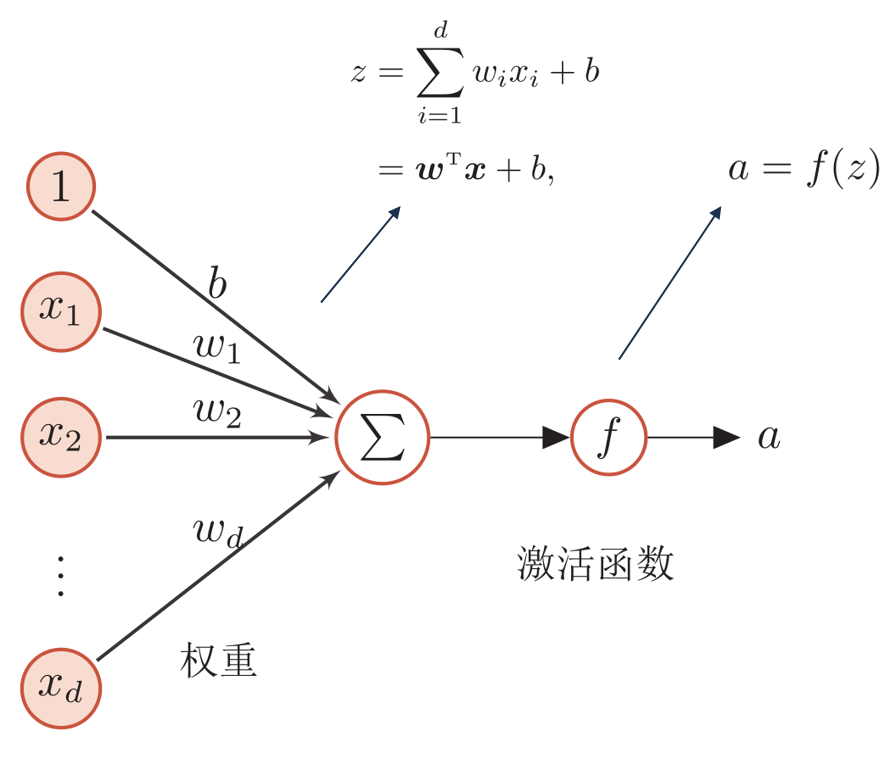
\includegraphics[width=0.6\linewidth]{人工神经元.png}
    \caption{人工神经元模型}
    \label{fig:神经元}
  \end{figure}

在图~\ref{fig:神经元}中,$\vec{x}$为输入向量,$w$和$b$分别是权重和偏移,

神经网络主要由以下几部分组成:
\begin{itemize}
    \item 输入节点(输入层)。在这一层中不进行任何计算,它们只是将信息传递给下一层(大部分时间是隐藏层)。
    \item 隐藏节点(隐藏层)。中间处理或计算在隐藏层中完成的,然后将输入层的权重(信号或信息)传递给下一层(另一个隐藏层或输出层)。一个神经网络也可以不包含隐藏层。
    \item 输出节点(输出层)。它是神经网络的最后一层,接收来自最后一个隐藏层的输入。通过激活函数可以得到合理范围内的理想数值,例如用于分类的softmax函数。
    \item 连接和权重。神经元之间会有边进行连接,每条边会有一定的权重。即每个连接将神经元$i$的输出传递给神经元$j$的输入,每个连接被赋予一个权重$W_{ij}$。
    \item 激活函数。激活函数负责为神经网络引入非线性特征。它把值压缩到一个更小范围,即一个 Sigmoid 激活函数的值区间为 [0,1]。深度学习中有很多激活函数,如Sigmoid、Tanh、ReLU 、Softplus、Softmax 等。下表为常见的激活函数。
    \begin{table}[]
        \caption{激活函数}
        \centering
        \begin{tabular}{|l|l|l|}
        \hline
        名称&表达式&导数\\ \hline
        Sigmoid &  $f(x) = \frac{1}{1+e^{-x}}$ & $f'(x) = f(x)(1-f(x))$
        \\ \hline
        Tanh & $f(x) = \frac{2}{1+e^{-2x}} - 1$ & $f'(x) = 1 - f(x)^2$ \\ \hline
        ReLU & $f(x) = max(0, x)$ & $f(x)=\begin{cases}
        0& \text{x<0}\\
        1& \text{x>=0}
        \end{cases}$ \\ \hline
        Softplus & $f(x) = log(1+e^x)$ & $f'(x) = \frac{1}{1+e^x}$ \\ \hline
        Softmax & $S_i = \frac{e_i}{\sum_j e_j}$ & \\ \hline
        \end{tabular}
        \end{table}
    \item 学习规则。学习规则是一种规则或算法,它修改神经网络的参数,以使网络的给定输入产生一个有利的输出。这个学习过程通常相当于修改权重和阈值。
\end{itemize}

\subsection{RNN}
RNN是一种针对时序数据处理的神经网络模型。相较于普通的神经网络模型来说,更擅长处理序列数据,即该网络其具有短期记忆能力。在循环神经网络中,神经元不但可以接受其他神经元的信息,也可以接受自身的信息,形成具有环路的网络结构。

循环神经网络的通用近似定理[Haykin, 2009]: 如果一个完全
连接的循环神经网络有足够数量的sigmoid 型隐藏神经元,它可以以任意
的准确率去近似任何一个非线性动力系统

% 神经网络有很多类型,这里本文将神经网络划分为前馈神经网络和循环神经网络,其中前馈神经网络包含单层感知机、多层感知机(MLP)、卷积神经网络(CNN)等。
% 本文主要介绍循环神经网络, 循环神经网络(Recurrent Neural Network,RNN)是一类具有短期记忆能力的神经网络。.和前馈神经网络相比,循环神经网络更加符合生物神经网络的结构。
下图~\ref{fig:循环神经网络}是循环神经网络的示意图。
\begin{figure}
    \centering
    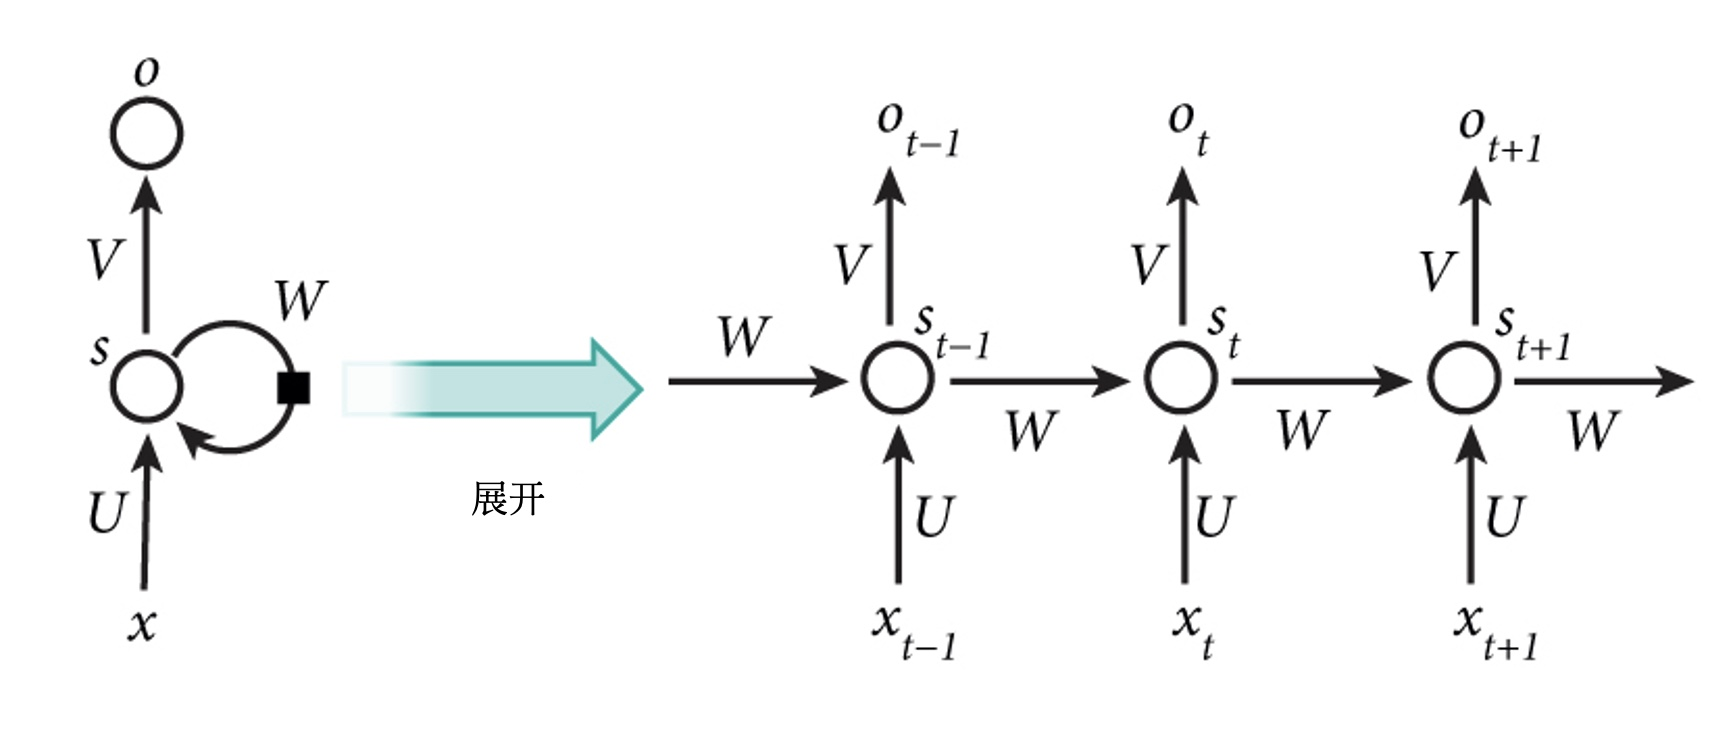
\includegraphics[width=0.6\linewidth]{循环神经网络.jpg}
    \caption{循环神经网络}
    \label{fig:循环神经网络}
  \end{figure}
该图显示了一个循环神经网络被展开成一个完整的神经网络。例如,如果输入序列是一个由5个单词组成的句子,那么网络就会被展开成一个5层神经网络,每个单词一层。这个网络在t时刻接收到输入 $x_t$ 之后,隐藏层的值是 $s_t$ ,输出值是 $o_t$ 。关键一点是, $x_t$ 的值不仅仅取决于 $s_t$ ,还取决于 $s_{t-1}$ 。
  用公式表示如下:
  \begin{equation}
      \begin{aligned}
          O_t &= g(V\cdot S_t) \\
          S_t &= f(U\cdot X_t + W\cdot S_{t-1})
      \end{aligned}
  \end{equation}

  $x_t$表示第$t$步的输入,例如$x_1$表示时刻1的特征向量。$s_t$表示第t步隐藏层状态,也就是网络中的“记忆”。$s_t$是由前一层的隐藏层状态和当前层的输入计算得到。函数$f(\cdot)$通常是一个非线性函数,如tanh或者ReLU。

\subsection{LSTM}
普通RNN有不能处理长依赖的问题,因此Hochreiter提出了一种长短期记忆网络-LSTM,以及它的变种,它是一种特殊的RNN,适用于学习长期依赖。现在LSTM已经被广泛应用于各个领域。

所有RNN都具有链式形式。在普通的RNN中,这种循环是一种非常简单的结构,比如简单的tanh层。
\begin{figure}
    \centering
    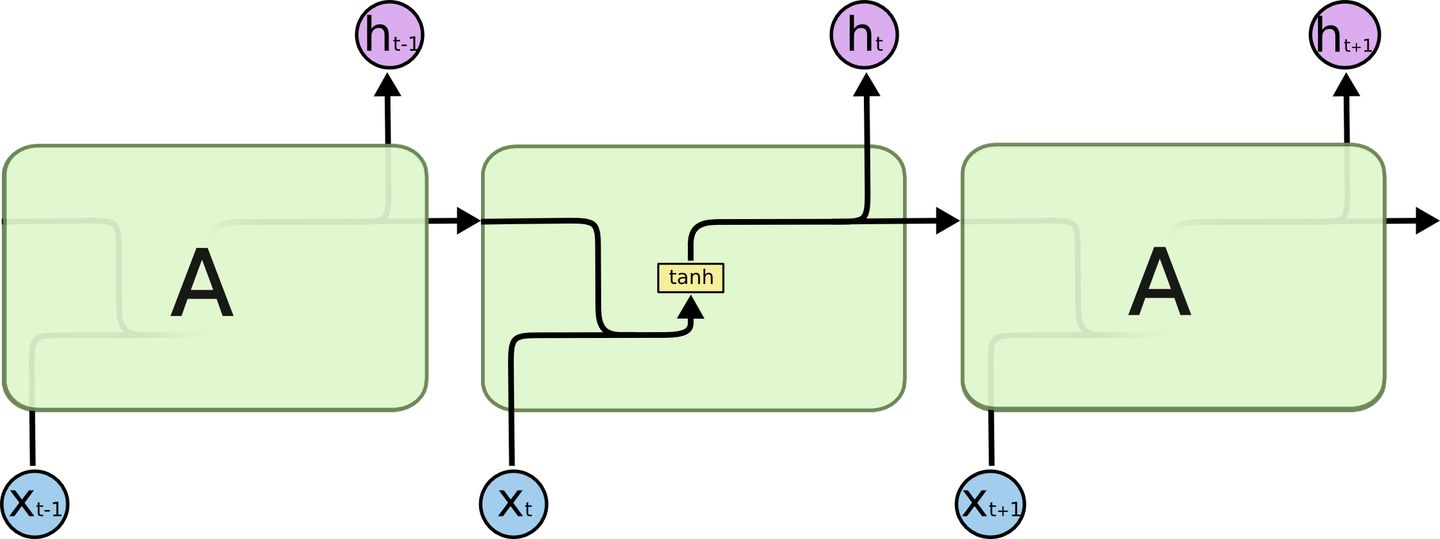
\includegraphics[width=0.6\linewidth]{普通RNN结构.jpg}
    \caption{普通RNN结构}
    \label{fig:普通RNN结构}
  \end{figure}

LSTM也具有这种链式结构,但循环单元里面不再是只有单一的神经网络层,而是构建了一些“门”(Gate)。原来的 RNN,由于这种链式结构的限制,很长的时刻以前的输入对现在的网络影响非常小,后向传播时那些梯度也很难影响很早以前的输入,即会出现梯度消失的问题。而 LSTM 通过构建“门”,让网络能记住那些非常重要的信息,比如遗忘门,来选择性清空过去的记忆和更新较新的信息。
\begin{figure}
    \centering
    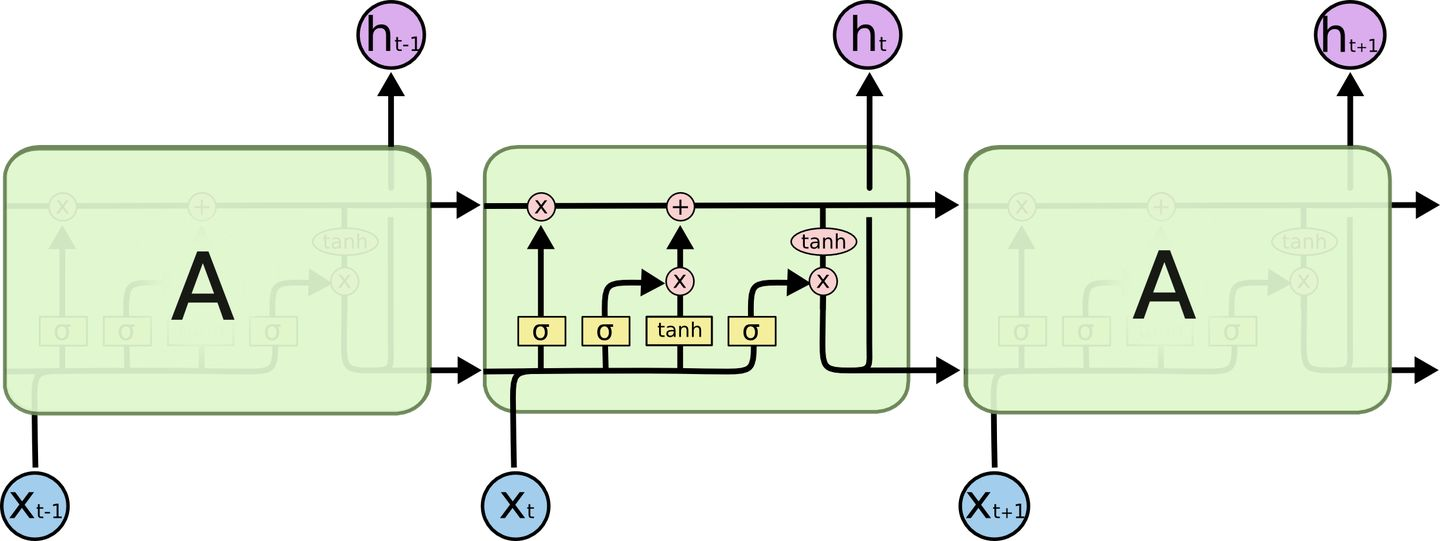
\includegraphics[width=0.6\linewidth]{LSTM结构.jpg}
    \caption{LSTM结构}
    \label{fig:LSTM结构}
  \end{figure}
  LSTM 中的第一步是决定从单元状态中丢弃什么信息。通过加入一个称为忘记门的$\sigma$层完成。遗忘门会读取上一时刻的输出$h_{t-1}$和当前时刻的输入$x_t$,计算出一个维度为n的向量$f_t$,该向量的值均在$(0, 1)$之间。1 表示“完全保留”上个神经元的状态信息,0 表示“完全舍弃”。

\begin{equation}
    \begin{aligned}
        f_t = \sigma(W_f\cdot x_t + U_f\cdot h_{t-1} + b_f)
    \end{aligned}
\end{equation}

下一步是确定该神经元的哪些新状态信息被存放在单元状态中。这里包含两个部分。第一,sigmoid 层,即 “输入门层” ,决定LSTM单元将更新哪些值。然后, tanh 层创建一个新的候选值$z_t$的向量,该向量可以加入到下一层单元状态中。

\begin{equation}
    \begin{aligned}
        i_t = \sigma(W_i\cdot[h_{t-1},x_t] + b_i)
    \end{aligned}
\end{equation}

\begin{equation}
    \begin{aligned}
        \widetilde {C_t} = tanh(W_C\cdot[h_{t-1},x_t]+b_C)
    \end{aligned}
\end{equation}
最后一步是将旧单元状态$c_{t-1}$更新为新状态$c_t$。把旧状态与遗忘门$f_t$相乘,丢弃掉之前需要丢弃的信息。接着与新状态进行相加。综合得出该神经元的输出的状态,也即更新单元的状态。
\begin{equation}
    \begin{aligned}
        C_t = f_t * C_{t-1} + i_t * \widetilde{C_t}
    \end{aligned}
\end{equation}

\subsection{GRU}
循环门单元(Gated Recurrent Unit,GRU),由 Cho, et al. (2014)提出。它组合了遗忘门和输入门到一个单独的“更新门”中。它也合并了cell state和hidden state,并且做了一些其他的改变。结果模型比标准LSTM模型更简单,
\begin{figure}
    \centering
    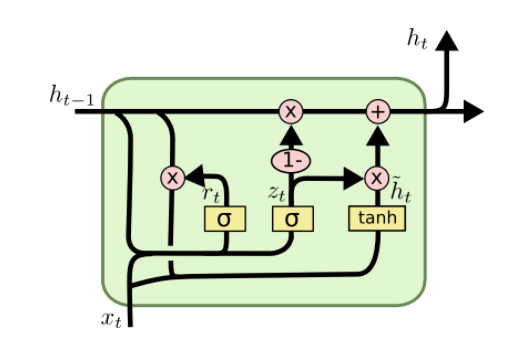
\includegraphics[width=0.6\linewidth]{GRU结构.png}
    \caption{GRU结构}
    \label{fig:GRU结构}
  \end{figure}

  \begin{equation}
    \begin{aligned}
        z_t = \sigma(W_z\cdot [h_{t-1},x_t])
    \end{aligned}
\end{equation}

\begin{equation}
    \begin{aligned}
        r_t = \sigma(W_r\cdot[h_{t-1},x_t])
    \end{aligned}
\end{equation}

\begin{equation}
    \begin{aligned}
        \widetilde {h_t} = tanh(W\cdot[r_t * h_{t-1}, x_t])
    \end{aligned}
\end{equation}

\begin{equation}
    \begin{aligned}
        h_t = (1- z_t) * h_{t-1} + z_t * \widetilde{h_t}
    \end{aligned}
\end{equation}
由图中结构可以看出,GRU是通过一个循环神经网络和“门”机制来不断更新内部参数,GRU算法的伪代码如下表所示。

\begin{algorithm}[!h]
    \caption{\emph{GRU}}
    \label{alg}
    \begin{algorithmic}[1]
      \Require
        t

      \Ensure
        内部参数
      \State 初始化t时刻单元状态
      \For{t $\leftarrow$ $1$ to $T$}
        $output_t$ = t
        $state_t$ = $output_t$
      \EndFor
    % %   \While {$\mathcal{L}$没有收敛}
    %       \State 利用公式 计算每一个节点$v$的$q_\phi(\bm{y}_v | \bm{A}, \bm{X}, Y_L)$以及$h_v^{K-1}$
    %       \For{i $\leftarrow$ $1$ to $m$}
    %       \State 从分布$q_\phi(Y_U | \bm{A}, \bm{X}, Y_L)$中采样$Y_U$
    %       \State 在采样得到的$Y_U$基础上,利用公式计算$q_\phi(\bm{z}| \bm{A}, \bm{X}, Y)$ 
    %        \For{j $\leftarrow$ $1$ to $n$}
    %        \State 从分布$q_\phi(\bm{z}| \bm{A}, \bm{X}, Y)$ 中采样$\bm{z}$
    %        \State 在采样得到的$\bm{z}$基础上用公式 计算$p_{\theta}(\bm{y}_v|\bm{A}, \bm{X}, \bm{z})$
    %        \EndFor
    %       \EndFor
    %       \State 用公式计算目标函数$\mathcal{L}(\theta, \phi)$ 
    %       \State 用梯度下降法更新$q_{net1}$,$q_{net2}$和$p_{net}$的所有参数
    %   \EndWhile
      %\State \Return $P_{net}$
    \end{algorithmic}
  \end{algorithm}

\begin{algorithm}[!h]
    \caption{\emph{LSTM层}}
    \begin{algorithmic}[1]
        \Require 一组按时间排列的向量组
        \Ensure 按时间排列的向量组
        \State $\vec C_0 = \vec 0$
        \State $\vec h_0 = \vec 0$
        \For{$t$ \leftarrow $1$ to $T$}


        \EndFor
    \end{algorithmic}
\end{algorithm}
  
$  state_t = 0
  for input_t in input_sequence:
    output_t = activation(dot(W, input_t) + dot(U, state_t) + b)
    state_t = output_t$
\section{基于图结构的RNN}
有向权重图$G=(V,E,W)$,$V$表示特征节点的集合,其中$|V|=N$, $E$表示特征间的关联关系,即图中的边,$W∈R[N*N]$为特征节点的相似度的加权邻接矩阵。将流量表示为G的一个图信号,P为每个节点特征数,则-时间t观察到的图信号。那么流量预测目的就是:给定G下,学得一个函数将T'个历史图信号映射到未来T时刻的图信号:
\begin{equation}
    h[X^{t-T+1}, X^{t-T+2},...,X^{t}; G] \Rightarrow [X^{t+1}, X^{t+2}, ..., X^{t+T}]
\end{equation}

\begin{equation}
    r^{(t)} = \sigma(\Theta_r\star G[X^{(t)},H^{t-1}] + b_r)
\end{equation}

\begin{equation}
    u^{(t)} = \sigma(\Theta_u\star G[X^{(t)},H^{t-1}] + b_u)
\end{equation}

\begin{equation}
    C^{(t)} = tanh(\Theta_C\star_G[X^{(t)},(r^{(t)}\odot H^{(t-1)})] + b_c)
\end{equation}

\begin{equation}
    H^{(t)} = u^{(t)}\odot H^{(t-1)} + (1 - u^{(t)}) \odot C^{(t)}
\end{equation}

其中$X^{(t)}$, $H^{(t)}$表示在时间 $t$ 的输入和输出,$r^{(t)}$ $u^{(t)}$分别是在时间 $t$的复位门和更新门。$\star_G$  表示在等式 2 中定义的扩散卷积,并且  是对应滤波器的参数。与GRU相似,DCGRU可用于构建递归神经网络层,并使用反向传播进行训练。

我们利用递归神经网络(RNN)对时间依赖性进行建模。特别是,我们使用门控循环单元(GRU)(Chung等,2014),它是RNN的简单而强大的变体。我们用扩散卷积代替了GRU中的矩阵乘法,这导致了我们提出的扩散卷积门控递归单元(DCGRU)。

\subsection{aa}
通常,计算卷积会很费时。 但是,如果$G$稀疏,则可以使用总时间复杂度 $O(K \mid \varepsilon \mid \ll O(N^ 2)$ 递归稀疏矩阵乘法来有效地计算方程2。


% 循环神经网络解决了这个问题。它们是带有循环的网络,允许信息持续存在。循环神经网络可以被认为是同一个网络的多个副本,每个副本都会向后继者传递信息。
\section{实验方案设计及实验流程}
\begin{equation*} hl=[hl_{1},\ hl_{2},\ \ldots,\ hl_{n-f+1}] \tag{-} \end{equation*}

\section{算法性能评估}

其中多分类任务的准确率指标为对于每个标签,分别计算precision,然后取不加权平均。$\mathbb{E}$

\begin{table*}[t]
    \small
    \caption{部分评估结果,待填充具体数值}
    \label{table2}
    \centering
    \begin{tabular}{c|c|ccc|ccc|cc}
    \toprule
    
     数据集 &  任务  &  
     LR &  NB & DT & CNN & CNN-LSTM & GRU & DCRNN-A & DCRNN-B \\
    \midrule
    % & 5\% & 79.87 & 80.61 & 79.08 & 81.69 & 78.05 & 75.80 & 82.21 & \textbf{82.49}\\
    
    % & 4\% &79.35 & 80.22 & 78.89 & 80.85 & 75.07 & 72.41 & 82.11 & \textbf{82.44} \\
    
    UNSW-NB15 & 二分类 & 0.848 & 79.33 & 78.52 &  80.51 & 62.74 & 68.91 & \textbf{82.69} & 81.66 \\ 
    
    & 多分类 &76.73 & 77.96 & 76.82 & 77.98 & 47.11 & 56.30 & \textbf{81.05} & 79.94 \\
    
    % & 1\% & 66.58 & 70.09 & 68.18 & 71.23 & 32.95 & 46.71 & \textbf{71.76} & 71.62 \\
    \midrule
    % & 5\%& 70.55 & 69.41 & 68.40 &  71.45 & 70.72 & 65.11 & 71.24 &  \textbf{71.89} \\
    % & 4\% & 69.11 & 68.33& 67.13 & 70.37 & 70.41 & 64.61 & 69.74 & \textbf{71.10} \\
    NSL-KDD & 二分类 & 68.26 & 67.11 & 65.54 & 70.18 & 65.04 & 58.49 & 70.26 & \textbf{70.88} \\
    & 多分类 & 67.01 & 67.37 & 66.41 & 68.31 & 56.16 & 53.18 & 68.47 & \textbf{70.24} \\
    % & 1\% & 60.08 & 61.39 & 61.25 & 63.25 & 30.28 & 49.57 & 62.21 & \textbf{64.91} \\
    \midrule
    % & 0.5\%& 82.18 & 80.01 & 81.32 &  78.25 & \textbf{82.73} & 78.97 & 82.17 & 80.70\\
    % & 0.4\%& 80.85 & 79.09 & 79.82 & 76.32 & 81.53 &  75.86 & \textbf{81.70} & 79.92\\
    CAMPUS & 二分类 & 79.98 & 77.95 & 79.51 & 75.62 & 79.80 & 75.25 & \textbf{80.69} & 79.10\\
    & 多分类 & 76.33 & 77.01 & 77.54 & 73.01 & 76.59 & 59.28 & 78.12 & \textbf{78.89}\\
    % & 0.1\% & 69.21 & 70.99 & 71.42 & 67.92 & 42.46 & 55.92 & 72.23 & \textbf{73.17}\\
    
     \bottomrule
    
    \end{tabular}
    \end{table*}

\subsection{基于开源数据集的检测结果}
% \begin{algorithm}
%     \caption{A}
%     \label{alg:A}
%     % \begin{algorithmic}
%     \STATE {set $r(t)=x(t)$} 
%     \REPEAT 
%     \STATE set $h(t)=r(t)$ 
%     \REPEAT
%     \STATE set $h(t)=r(t)$ 
%     \UNTIL{B} 
%     \UNTIL{B}
%     % \end{algorithmic}
%     \end{algorithm}
\begin{algorithm}[!h]
    \caption{\emph{GRNN}}
    \label{alg}
    \begin{algorithmic}[1]
      \Require
        一组按时间排序的向量组$\vec{x_1}$,$\vec{x_2}$,...,$\vec{x_T}$, 特征间关系图$G$以及它的邻接矩阵$W$

      \Ensure
        按时间排序的向量组$\vec{h_1}$,$\vec{h_2}$,...,$\vec{h_T}$
      \State 通过Xavier方法初始化$q_{net1}$, $q_{net2}$ and $p_{net}$的所有参数
      \While {$\mathcal{L}$没有收敛}
          \State 利用公式 计算每一个节点$v$的$q_\phi(\bm{y}_v | \bm{A}, \bm{X}, Y_L)$以及$h_v^{K-1}$
          \For{i $\leftarrow$ $1$ to $m$}
          \State 从分布$q_\phi(Y_U | \bm{A}, \bm{X}, Y_L)$中采样$Y_U$
          \State 在采样得到的$Y_U$基础上,利用公式计算$q_\phi(\bm{z}| \bm{A}, \bm{X}, Y)$ 
           \For{j $\leftarrow$ $1$ to $n$}
           \State 从分布$q_\phi(\bm{z}| \bm{A}, \bm{X}, Y)$ 中采样$\bm{z}$
           \State 在采样得到的$\bm{z}$基础上用公式 计算$p_{\theta}(\bm{y}_v|\bm{A}, \bm{X}, \bm{z})$
           \EndFor
          \EndFor
          \State 用公式计算目标函数$\mathcal{L}(\theta, \phi)$ 
          \State 用梯度下降法更新$q_{net1}$,$q_{net2}$和$p_{net}$的所有参数
      \EndWhile
      %\State \Return $P_{net}$
    \end{algorithmic}
  \end{algorithm}




%   \begin{algorithm}[!h]
%     \caption{\emph{GSNN}}
%     \label{alg}
%     \begin{algorithmic}[1]
%       \Require
%         图$G$以及它的邻接矩阵$A$,节点特征矩阵$X$以及已知节点的标签信息$T_L$,采样得到的$Y_U$和$\bm{z}$的数量:$m$和$n$

%       \Ensure
%         优化后的$q_{net1}$, $q_{net2}$和$p_{net}$所有参数
%       \State 通过Xavier方法\cite{glorot2010understanding}初始化$q_{net1}$, $q_{net2}$ and $p_{net}$的所有参数
%       \While {$\mathcal{L}$没有收敛}
%           \State 利用公式 \ref{seven} 计算每一个节点$v$的$q_\phi(\bm{y}_v | \bm{A}, \bm{X}, Y_L)$以及$h_v^{K-1}$
%           \For{i $\leftarrow$ $1$ to $m$}
%           \State 从分布$q_\phi(Y_U | \bm{A}, \bm{X}, Y_L)$中采样$Y_U$
%           \State 在采样得到的$Y_U$基础上,利用公式 \ref{eight}计算$q_\phi(\bm{z}| \bm{A}, \bm{X}, Y)$ 
%            \For{j $\leftarrow$ $1$ to $n$}
%            \State 从分布$q_\phi(\bm{z}| \bm{A}, \bm{X}, Y)$ 中采样$\bm{z}$
%            \State 在采样得到的$\bm{z}$基础上用公式\ref{nine} 计算$p_{\theta}(\bm{y}_v|\bm{A}, \bm{X}, \bm{z})$
%            \EndFor
%           \EndFor
%           \State 用公式\ref{ten}计算目标函数$\mathcal{L}(\theta, \phi)$ 
%           \State 用梯度下降法更新$q_{net1}$,$q_{net2}$和$p_{net}$的所有参数
%       \EndWhile
%       %\State \Return $P_{net}$
%     \end{algorithmic}
%   \end{algorithm}

\subsection{基于真实数据的检测结果}
交叉熵损失函数经常用于分类问题中,特别是在神经网络做分类问题时,也经常使用交叉熵作为损失函数,此外,由于交叉熵涉及到计算每个类别的概率,所以交叉熵几乎每次都和sigmoid(或softmax)函数一起出现。

我们用神经网络最后一层输出的情况,来看一眼整个模型预测、获得损失和学习的流程:

神经网络最后一层得到每个类别的得分scores;
该得分经过sigmoid(或softmax)函数获得概率输出;
模型预测的类别概率输出与真实类别的one hot形式进行交叉熵损失函数的计算。

\chapter{流量检测系统的设计与实现}
本文实现的流量异常检测系统按照功能需求可以分为三个模块:数据采集和分析模块,异常检测模块,终端预警模块。

\begin{figure}
    \centering
    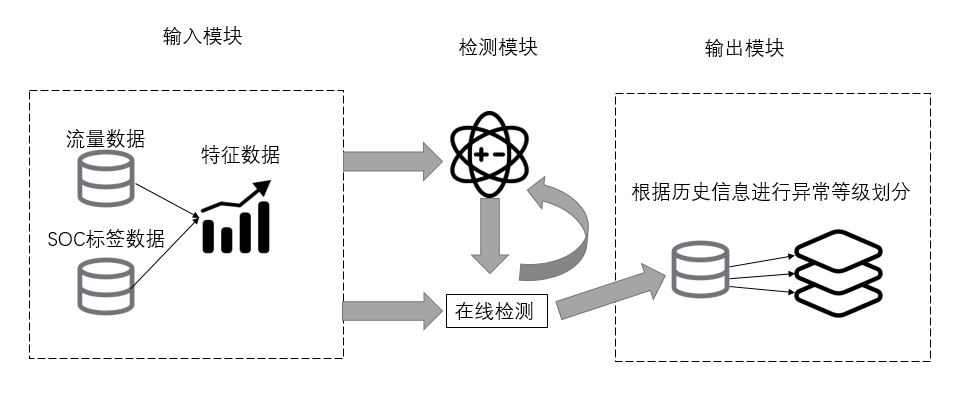
\includegraphics[scale=0.6]{系统架构图.png}
    % 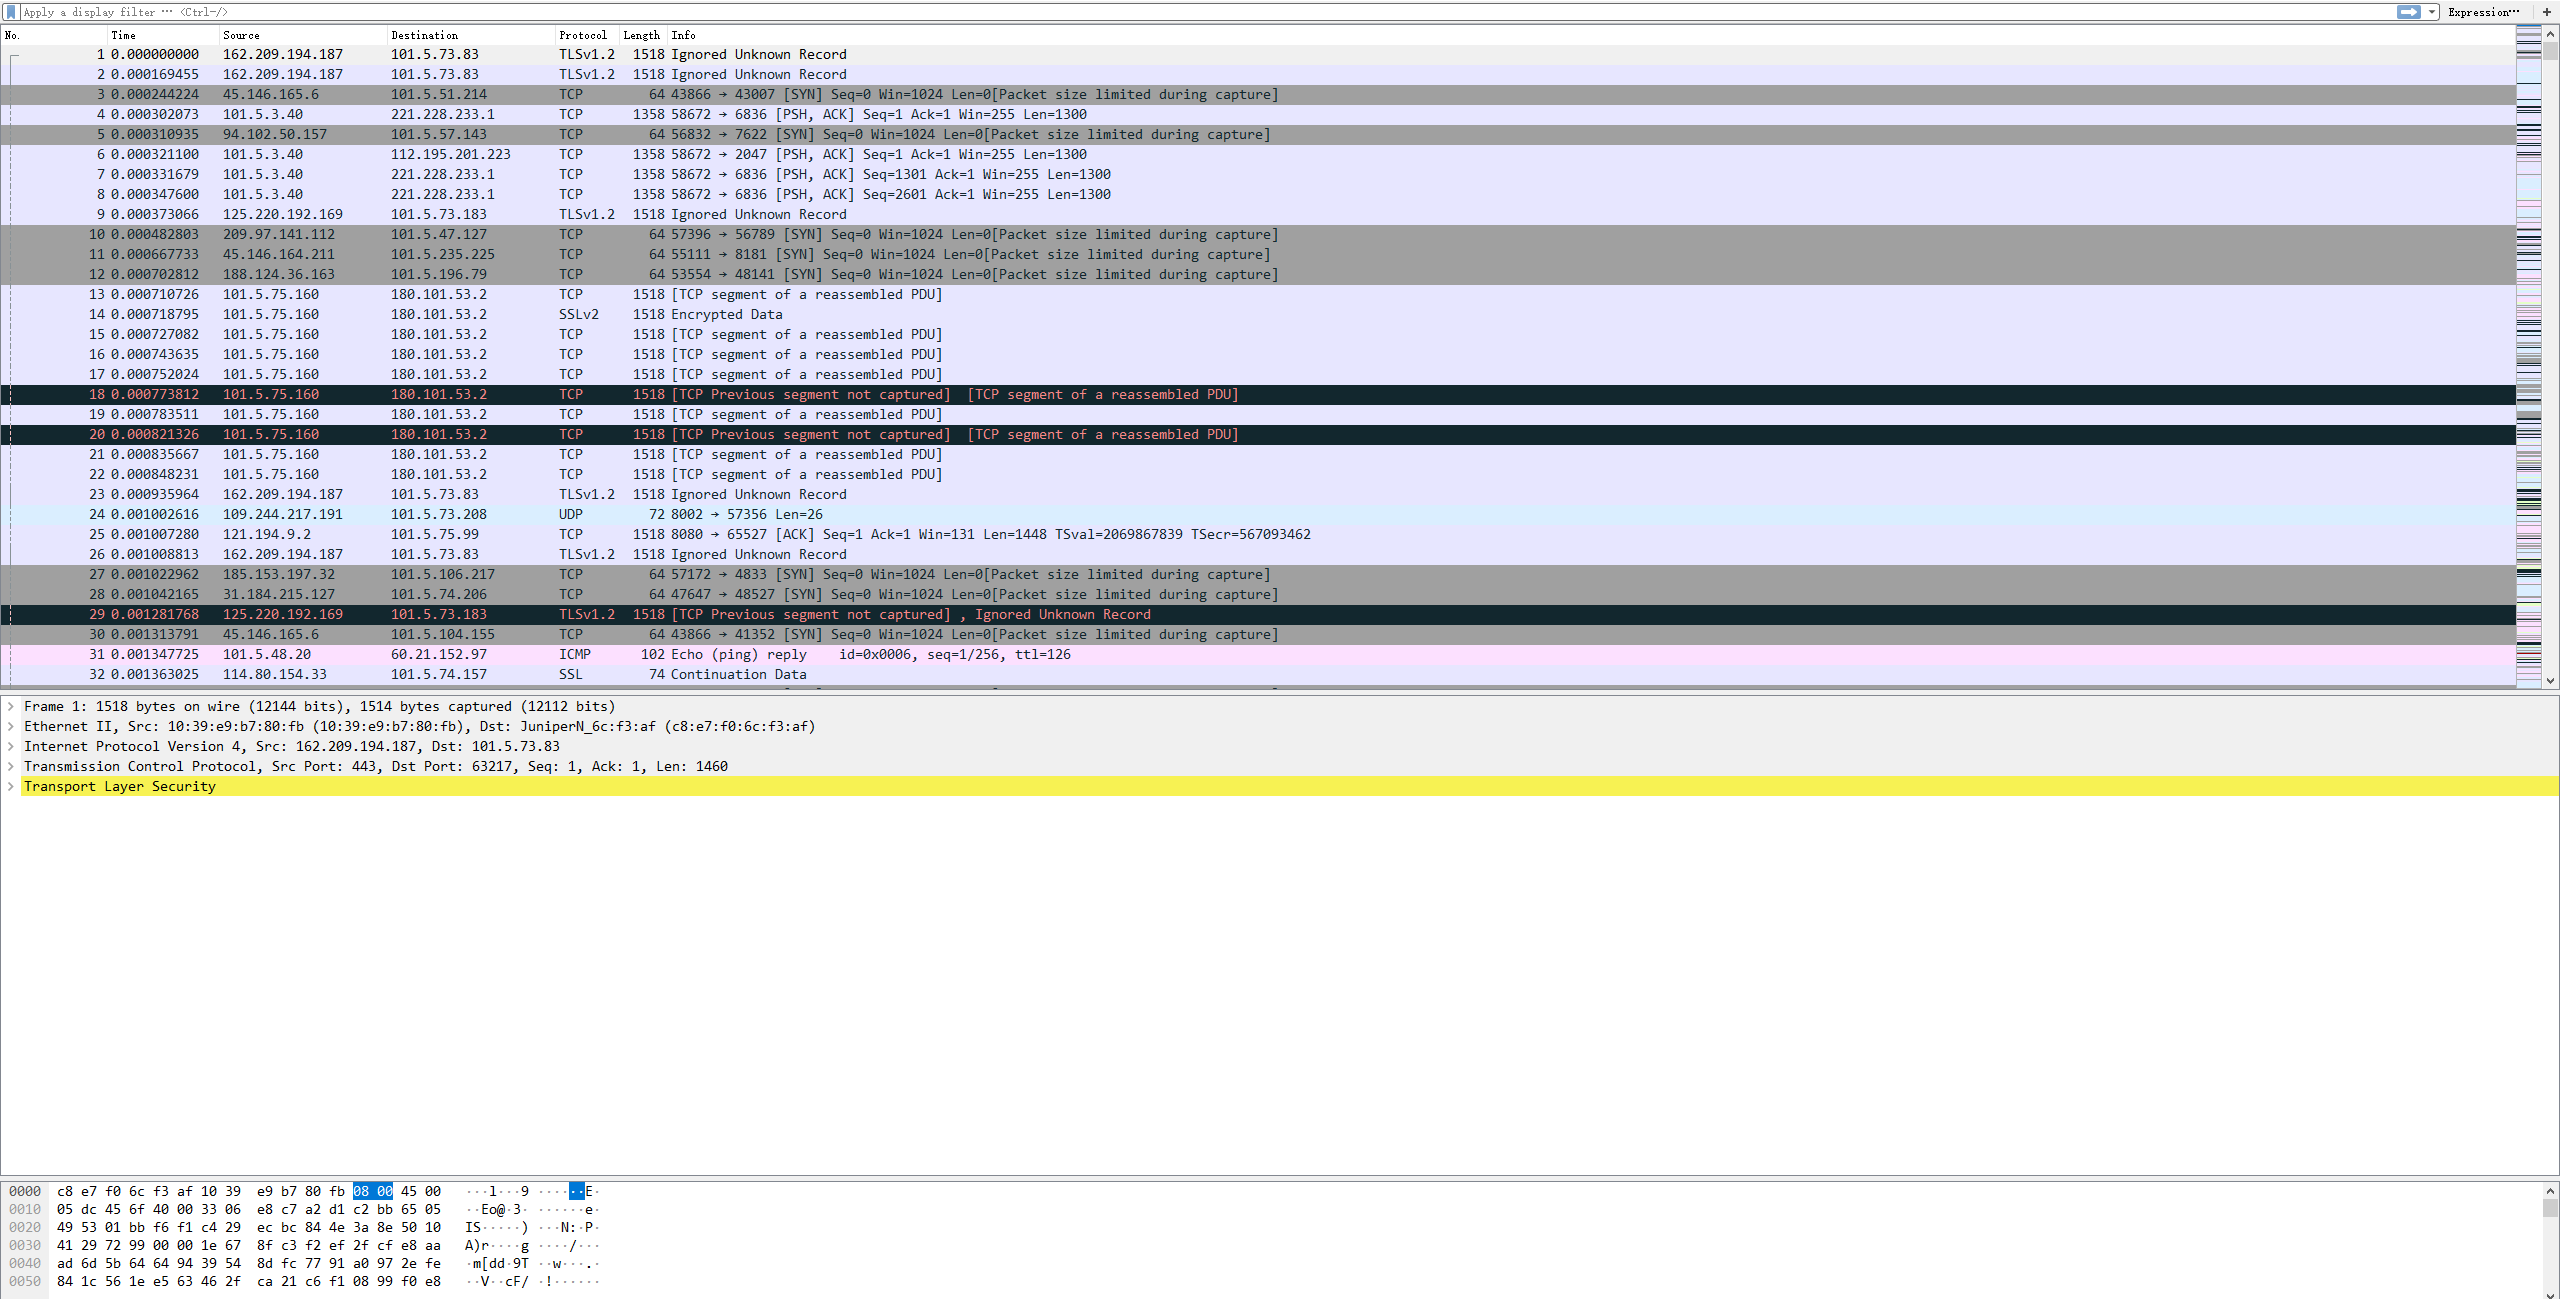
\includegraphics[width=0.6\linewidth]{wireshark流量图.png}
    \caption{系统架构图}
    \label{fig:arch}
  \end{figure}

\section{引言}
下面是对各个模块的介绍:

待补充。

% \section{使用大数据平台应对大规模流量的必要性}
\section{spark 平台介绍}
Spark 是 UC Berkeley AMP Lab 开源的通用分布式并行计算框架,目前已成为 Apache 软件基金会的顶级开源项目。Spark 支持多种编程语言,包括 Java、Python、R 和 Scala,同时 Spark 也支持 Hadoop 的底层存储系统 HDFS,但 Spark 不依赖 Hadoop。

Spark 基于 Hadoop MapReduce 算法实现的分布式计算,拥有 Hadoop MapReduce 所具有的优点,并且具有更高的运算速度。Spark 能够比 Hadoop 运算更快,主要原因是:Hadoop 在一次 MapReduce 运算之后,会将数据的运算结果从内存写入到磁盘中,第二次 MapReduce 运算时在从磁盘中读取数据,两次对磁盘的操作,增加了多余的 IO 消耗;而 Spark 则是将数据一直缓存在内存中,运算时直接从内存读取数据,只有在必要时,才将部分数据写入到磁盘中。除此之外,Spark 使用最先进的 DAG(Directed Acyclic Graph,有向无环图)调度程序、查询优化器和物理执行引擎,在处理批量处理以及处理流数据时具有较高的性能。按照Spark 官网的说法,Spark 相对于 Hadoop 而言,Spark 能够达到 100 倍以上的运行负载。

Spark Core是 Spark 的核心,主要负责任务调度等管理功能。Spark
Core 的实现依赖于 RDDs(Resilient Distributed Datasets,
弹性分布式数据集)的程序抽象概念。

Spark Streaming:这个模块主要是对流数据的处理,支持流数据的可伸缩和容错处理,可以与 Flume(针对数据日志进行优化的一个系统)和 Kafka(针对分布式消息传递进行优化的流处理平台)等已建立的数据源集成。Spark Streaming 的实现,也使用 RDD 抽象的概念,使得在为流数据(如批量历史日志数据)编写应用程序时,能够更灵活,也更容易实现。

Spark 有多种运行模式, Spark 支持本地运行模式(Local 模式)、独立运行模式(Standalone 模式)、Mesos、YARN(Yet Another Resource Negotiator)、Kubernetes 模式等。

本地运行模式是 Spark 中最简单的一种模式,也可称作伪分布式模式。本文中的系统就是使用的本地运行模式。

独立运行模式为 Spark 自带的一种集群管理模式,Mesos 及 YARN 两种模式也是比较常用的集群管理模式。相比较 Mesos 及 YARN 两种模式而言,独立运行模式是最简单,也最容易部署的一种集群运行模式。


Spark 底层还支持多种数据源,能够从其它文件系统读取数据,如 HDFS、Amazon S3、Hypertable、HBase 等。Spark 对这些文件系统的支持,同时也丰富了整个 Spark 生态的运行环境。

Spark 支持多种分布式部署模式,主要支持三种部署模式,分别是:Standalone、Spark on YARN和 Spark on Mesos模式。

Standalone模式为 Spark 自带的一种集群管理模式,即独立模式,自带完整的服务,可单独部署到一个集群中,无需依赖任何其他资源管理系统。它是 Spark 实现的资源调度框架,其主要的节点有 Driver 节点、Master 节点和 Worker 节点。Standalone模式也是最简单最容易部署的一种模式。

Spark on YARN模式,即 Spark 运行在Hadoop YARN框架之上的一种模式。Hadoop YARN(Yet Another Resource
Negotiator,另一种资源协调者)是一种新的 Hadoop 资源管理器,它是一个通用资源管理系统,可为上层应用提供统一的资源管理和调度。

Spark on Mesos模式,即 Spark 运行在Apache Mesos框架之上的一种模式。Apache Mesos是一个更强大的分布式资源管理框架,负责集群资源的分配,它允许多种不同的框架部署在其上,包括YARN。它被称为是分布式系统的内核。

三种架构都采用了Master/Worker(Slave)的架构,Spark 分布式运行架构大致如下:
\begin{figure}
    \centering
    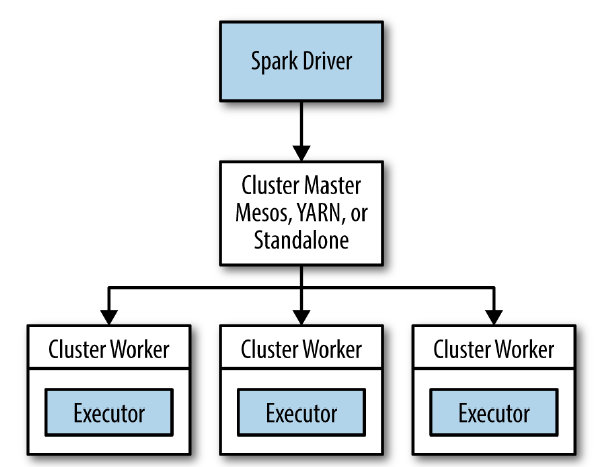
\includegraphics[scale=0.6]{spark分布式运行架构.jpg}
    % 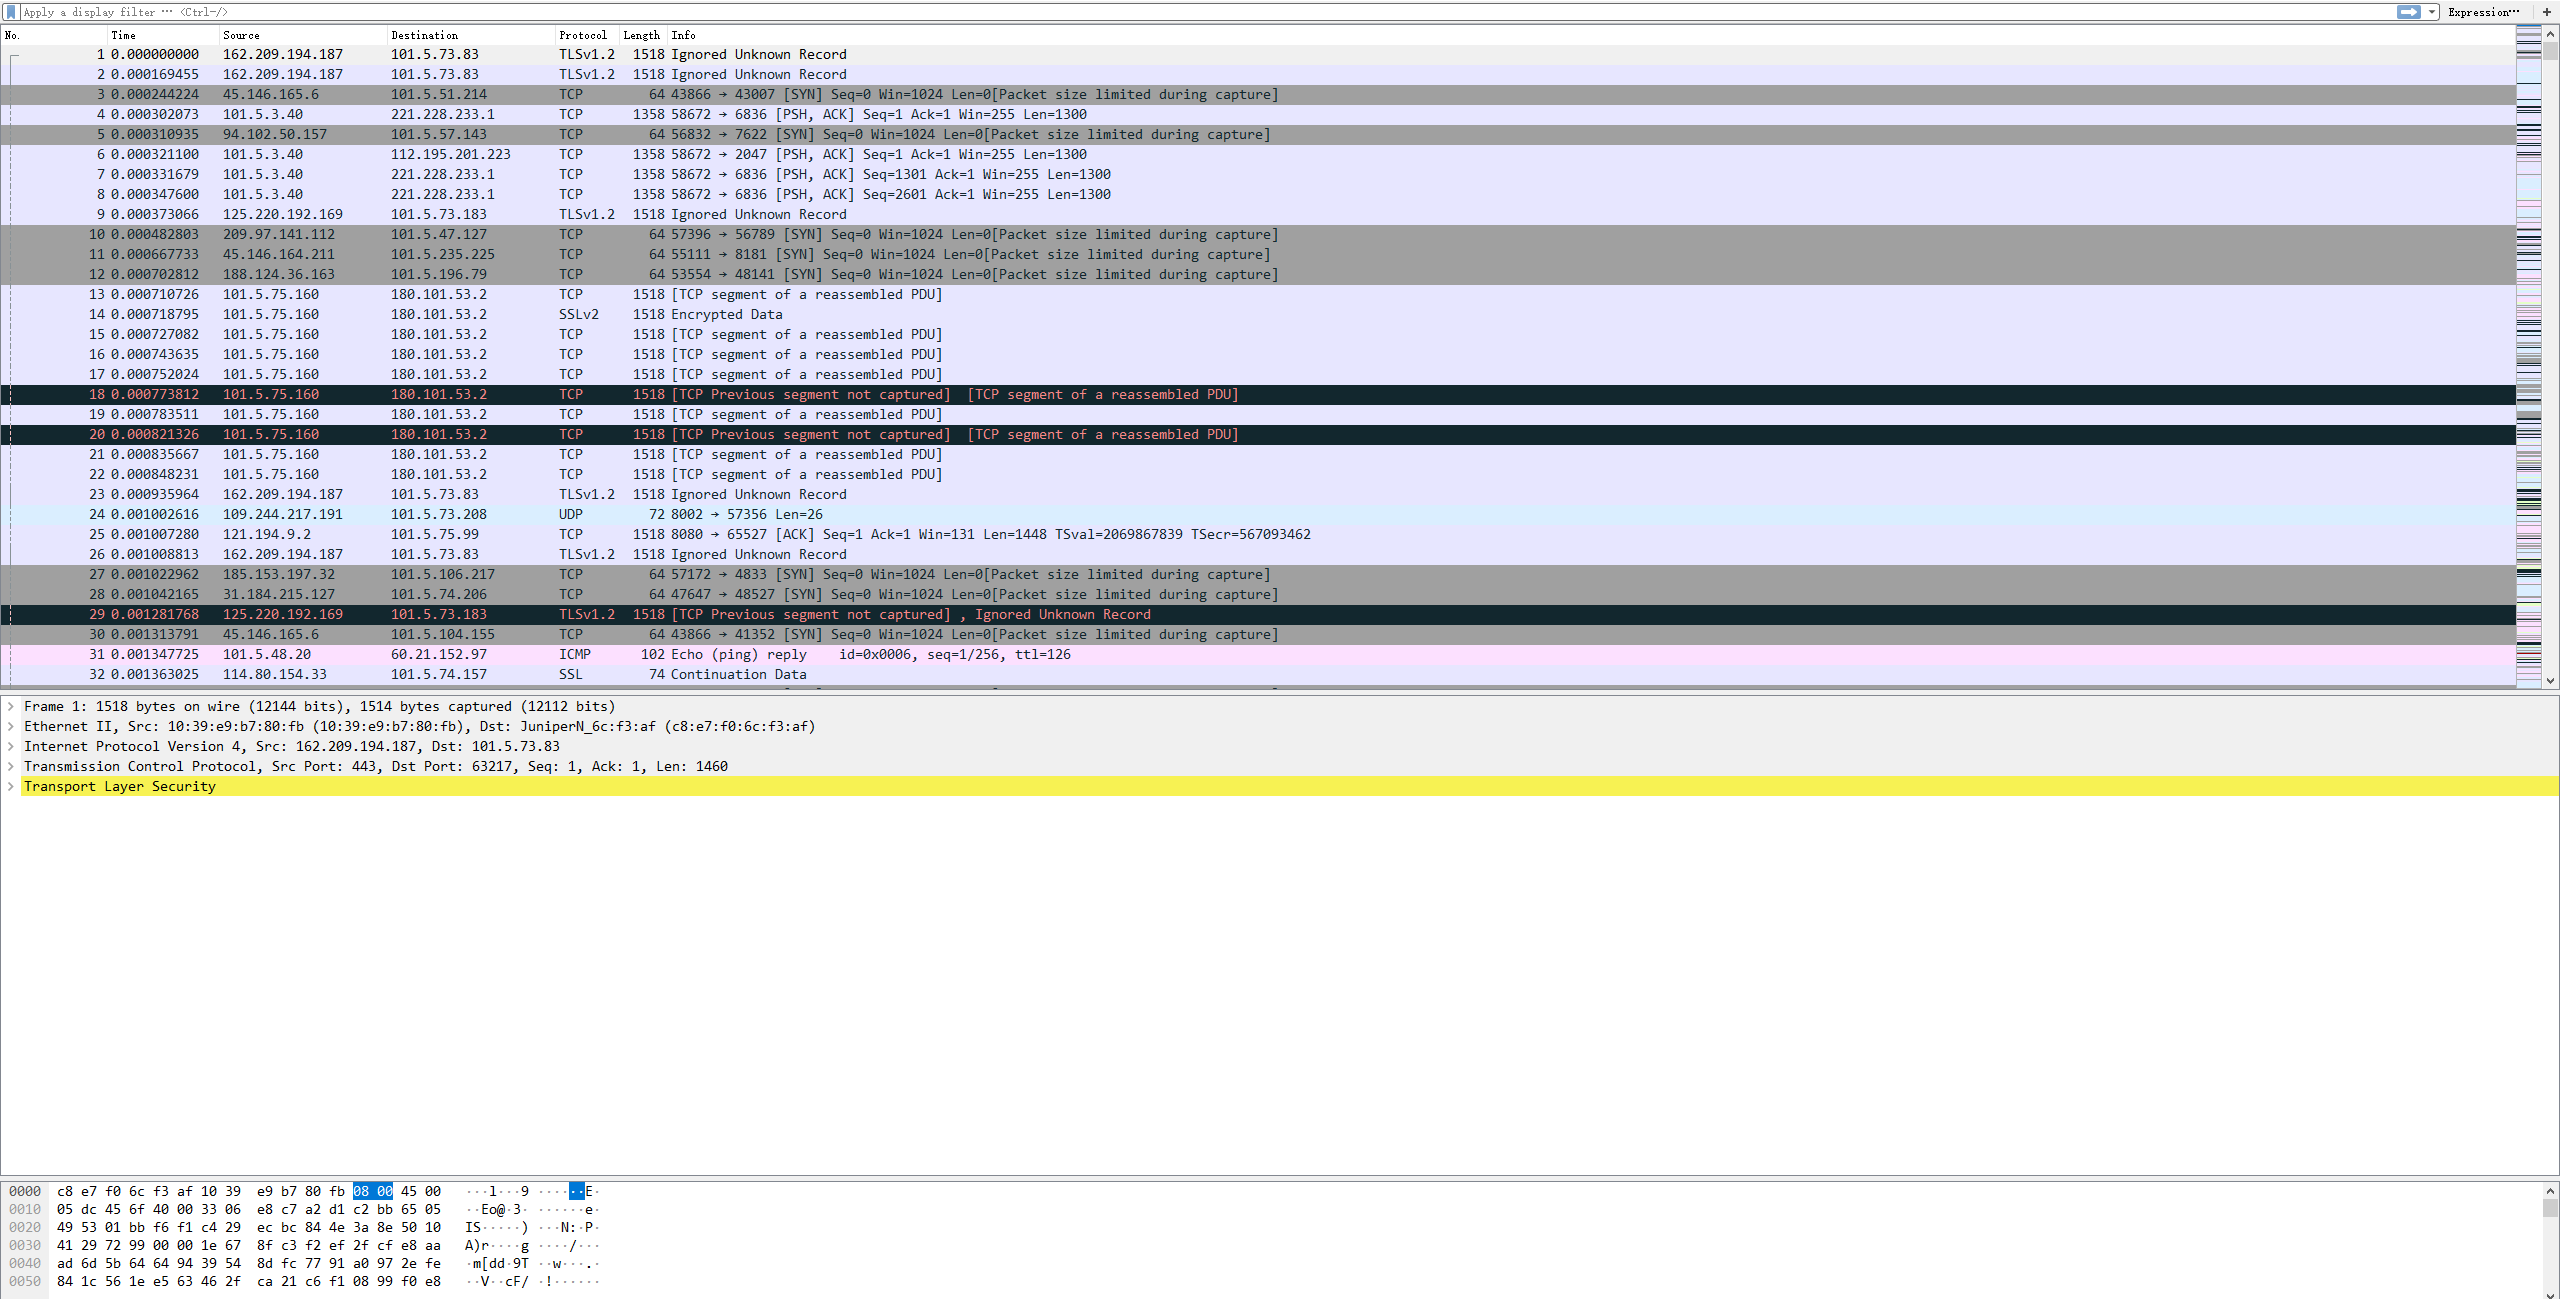
\includegraphics[width=0.6\linewidth]{wireshark流量图.png}
    \caption{spark分布式运行架构}
    \label{fig:spark}
  \end{figure}

  运行一个Spark Streaming应用程序,有下面一些步骤

  有管理器的集群-这是任何Spark应用程序都需要的需求,详见部署指南
  将应用程序打为jar包-你必须编译你的应用程序为jar包。如果你用spark-submit启动应用程序,你不需要将Spark和Spark Streaming打包进这个jar包。如果你的应用程序用到了高级源(如kafka,flume),你需要将它们关联的外部artifact以及它们的依赖打包进需要部署的应用程序jar包中。例如,一个应用程序用到了TwitterUtils,那么就需要将$spark-streaming-twitter_2.10$以及它的所有依赖打包到应用程序jar中。
  为executors配置足够的内存-因为接收的数据必须存储在内存中,executors必须配置足够的内存用来保存接收的数据。注意,如果你正在做10分钟的窗口操作,系统的内存要至少能保存10分钟的数据。所以,应用程序的内存需求依赖于使用它的操作。
  配置checkpointing-如果stream应用程序需要checkpointing,然后一个与Hadoop API兼容的容错存储目录必须配置为检查点的目录,流应用程序将checkpoint信息写入该目录用于错误恢复。
  配置应用程序driver的自动重启-为了自动从driver故障中恢复,运行流应用程序的部署设施必须能监控driver进程,如果失败了能够重启它。不同的集群管理器,有不同的工具得到该功能
  
  Spark Standalone:一个Spark应用程序driver可以提交到Spark独立集群运行,也就是说driver运行在一个worker节点上。进一步来看,独立的集群管理器能够被指示用来监控driver,并且在driver失败(或者是由于非零的退出代码如exit(1),或者由于运行driver的节点的故障)的情况下重启driver。
  YARN:YARN为自动重启应用程序提供了类似的机制。
  Mesos: Mesos可以用Marathon提供该功能
  
  配置write ahead logs-在Spark 1.2中,为了获得极强的容错保证,我们引入了一个新的实验性的特性-预写日志(write ahead logs)。如果该特性开启,从receiver获取的所有数据会将预写日志写入配置的checkpoint目录。这可以防止driver故障丢失数据,从而保证零数据丢失。这个功能可以通过设置配置参数spark.streaming.receiver.writeAheadLogs.enable为true来开启。然而,这些较强的语义可能以receiver的接收吞吐量为代价。这可以通过并行运行多个receiver增加吞吐量来解决。另外,当预写日志开启时,Spark中的复制数据的功能推荐不用,因为该日志已经存储在了一个副本在存储系统中。可以通过设置输入DStream的存储级别为StorageLevel.$MEMORY_AND_DISK_SER$获得该功能。

安装环境介绍(待补充):
本文将 Spark 部署在安装有 ubuntu16.04 系统的 VirtualBox 虚拟机中。

搭建 Spark 集群,需要准备以下文件及环境:
jdk-8u211-linux-x64.tar.gz
spark-2.4.3-bin-hadoop2.7.tgz
3 个独立的 ubuntu16.04 虚拟机系统,机器集群规划如下:

\section{spark streaming介绍}
Spark Streaming是Spark Core为支持流式处理的扩展,具有高容错,高吞吐的特点。
Spark Streaming在Spark Core的基础上继续实现StreamingContext(负责管理Spark Streaming程序运行的环境),JobSchedule(负责调度Job任务),JobGenerator(负责生成
Job任务),Receiver(负责接收数据)组件。

Spark Streaming内部的基本工作原理如下~\ref{fig:spark工作原理},接收实时输入数据流,然后将数据拆分成多个batch,比如每收集1秒的数据封装为一个batch,然后将每个batch交给Spark的计算引擎进行处理,最后会生产出一个结果数据流,其中的数据,也是由一个一个的batch所组成的。

\begin{figure}
    \centering
    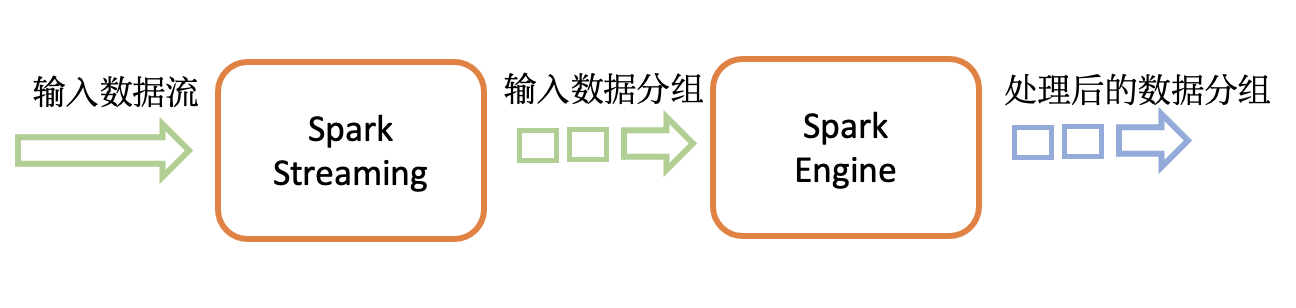
\includegraphics[scale=0.6]{spark工作原理.png}
    % 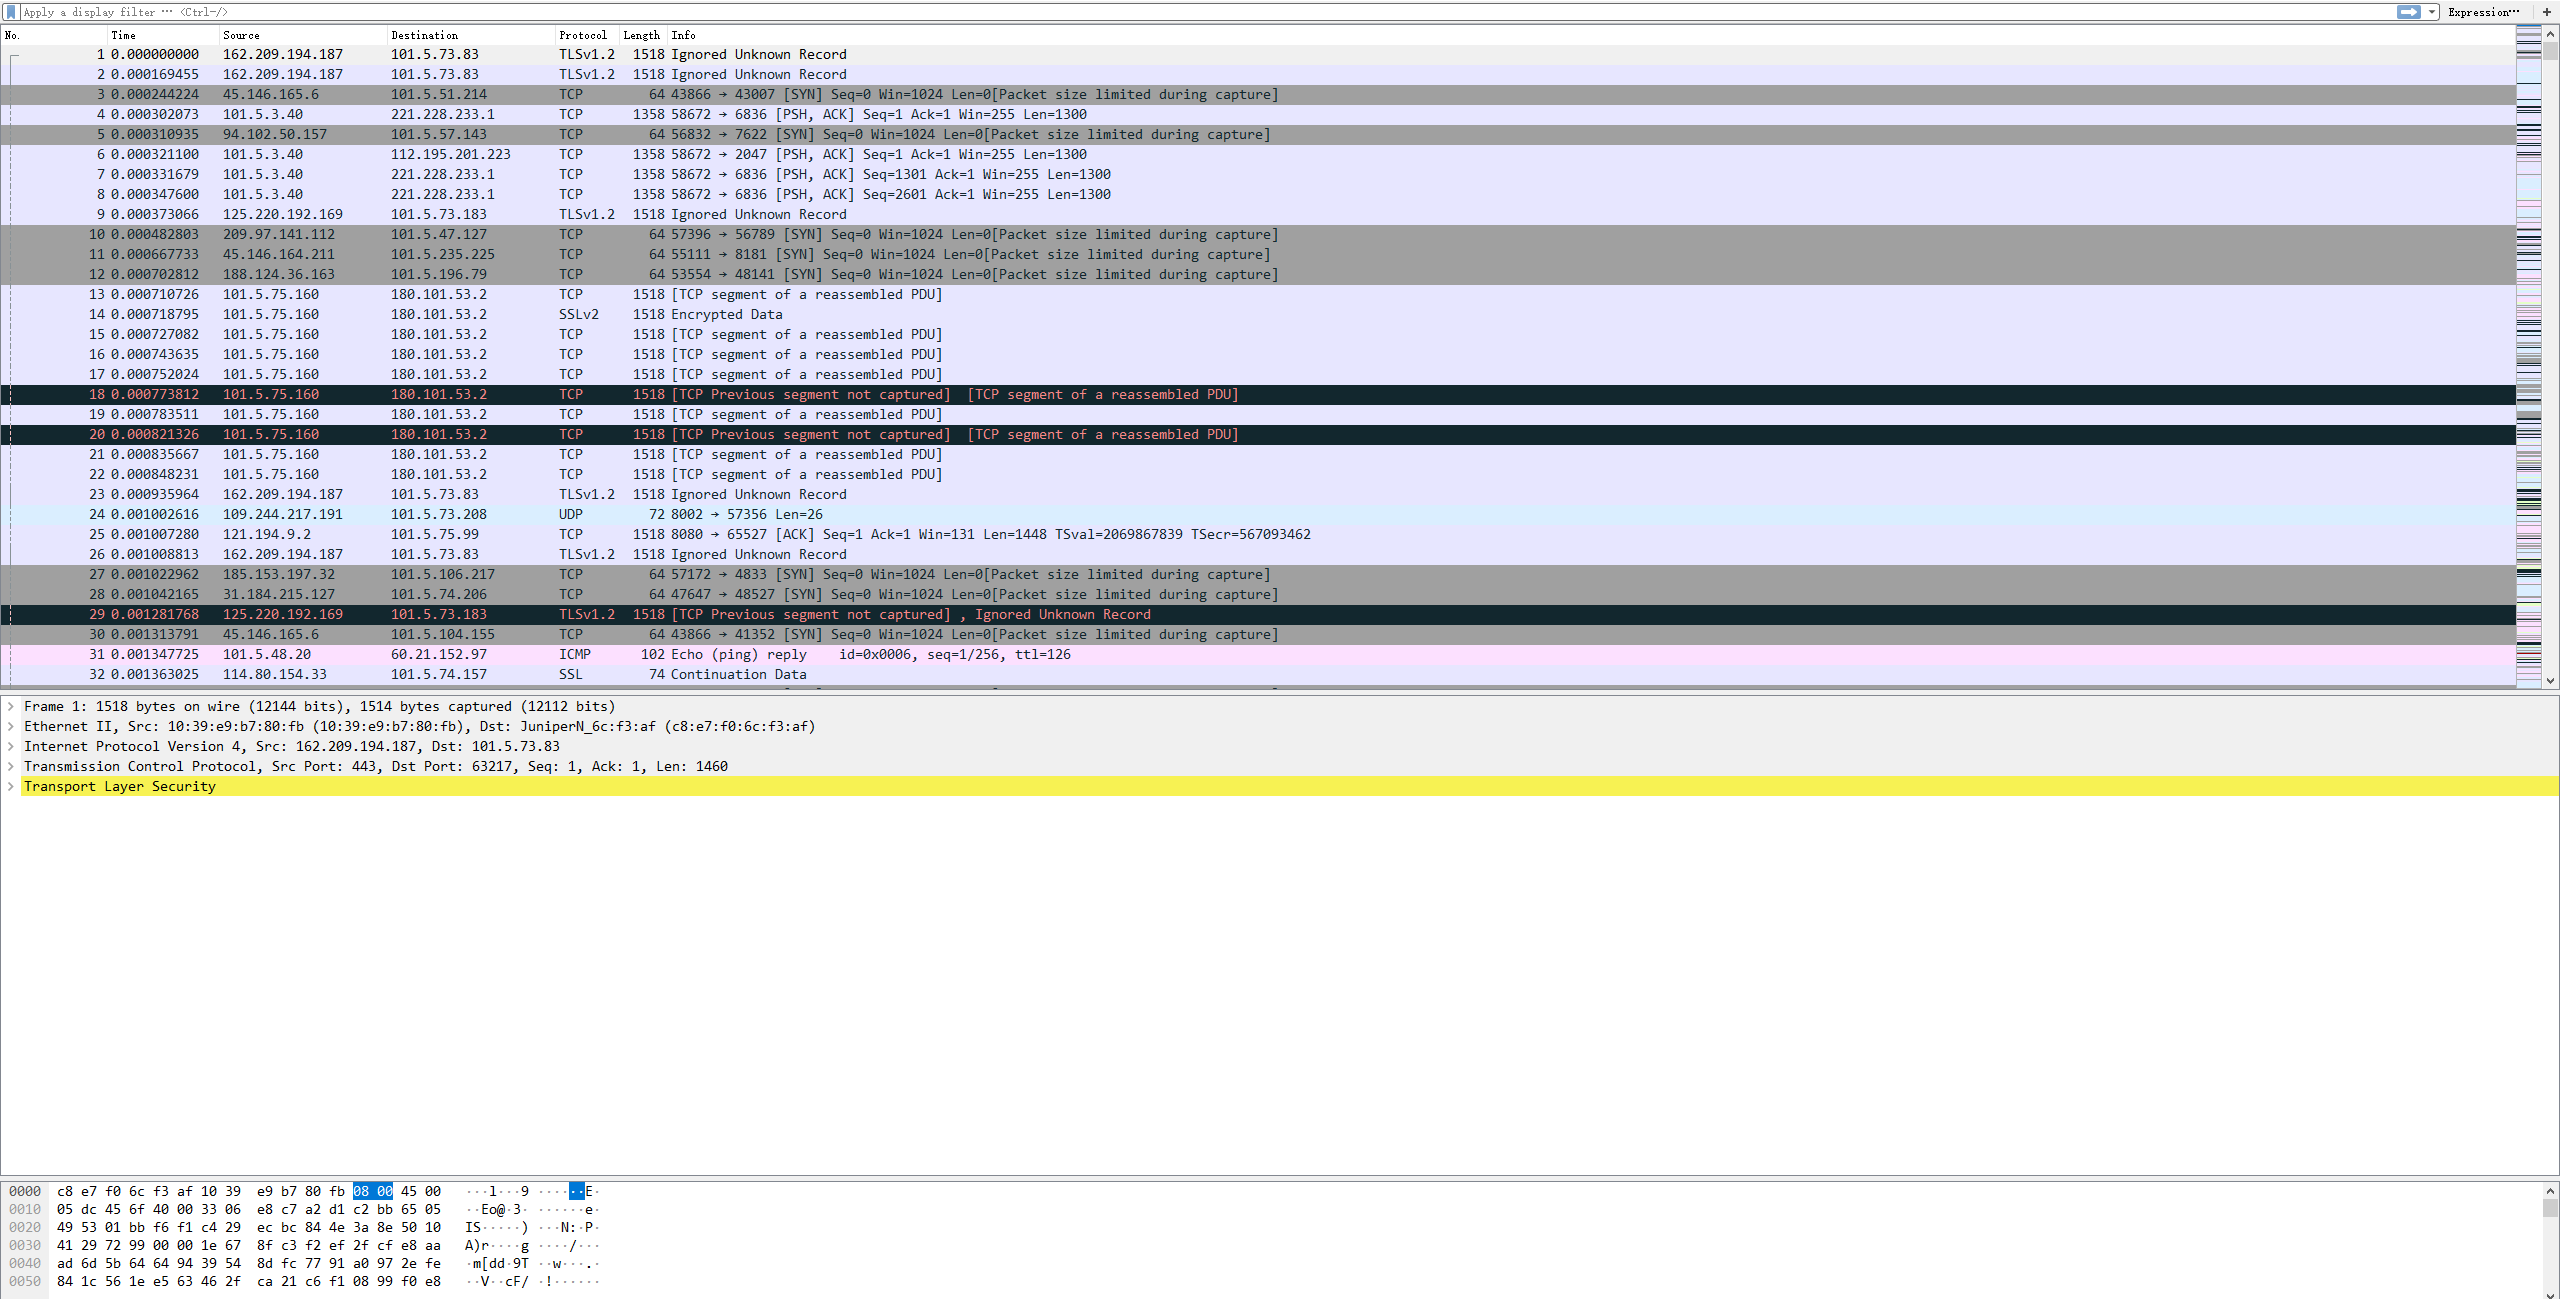
\includegraphics[width=0.6\linewidth]{wireshark流量图.png}
    \caption{spark工作原理}
    \label{fig:spark工作原理}
  \end{figure}

DStream是Spark Streaming中对数据流的一个抽象。DStream以哈希表的方式保存一
系列连续的RDD,哈希表的键是时间,值是RDD。随着时间的推移,DStream中产生新
的RDD,形成一个RDD流,但是由于RDD还是批处理方式,而且往往RDD中的数据量相
对较小,所以SparkStreaming对于数据的处理又称为微批处理。此外DStream和RDD—样,
提供map、foreach、flatMap、transform等算子。

Spark Streaming支持基本数据源和高级数据源,其中基本数据源包括hdfs(hadoop File System)文件源,简单socket源等,高级数据源包括kafka,Flume等。Spark Streaming
在执行的过程可以分成两个阶段,数据准备阶段和数据计算阶段,以下分别介绍。

下图~\ref{fig:spark}展示Spark Streaming接收数据的示意图,其中BlockGenerator,Receiver都是
Spark Streaming实现的组件,blockForPushing是一个阻塞队列。在Spark Streaming数
据准备阶段,首先Receiver从外部数据源接收数据并且将数据写入BlockGenerator的
ArrayBuffer(内存数组)中,该过程会保证数据接收速率始终小于设置的最大速率
maxRate,这个maxRate也可以由Spark的反压模块根据Spark集群的处理速度自行计算。
然后,BlockGenerator包含定时器Timer会定时将ArrayBuffer中的数据生成Block对象(块
对象,其中包含生成的数据),并且将Block对象写入BlockForPushing阻塞队列中,然后
再通知SparkStreaming的Driver程序,将Block对象分配至Block队列。最终,数据在Block
队列中等待Spark Streaming的计算阶段。以上便是Spark Streaming接收数据的全部过程。
\begin{figure}
    \centering
    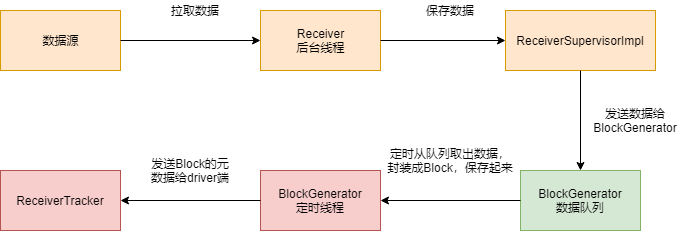
\includegraphics[scale=0.6]{spark数据源.png}
    \caption{Spark数据源}
    \label{fig:spark}
  \end{figure}

  下图~\ref{fig:spark streaming}是Spark Streaming作业的执行流程,具体流程分为以下几步:
  \begin{figure}
    \centering
    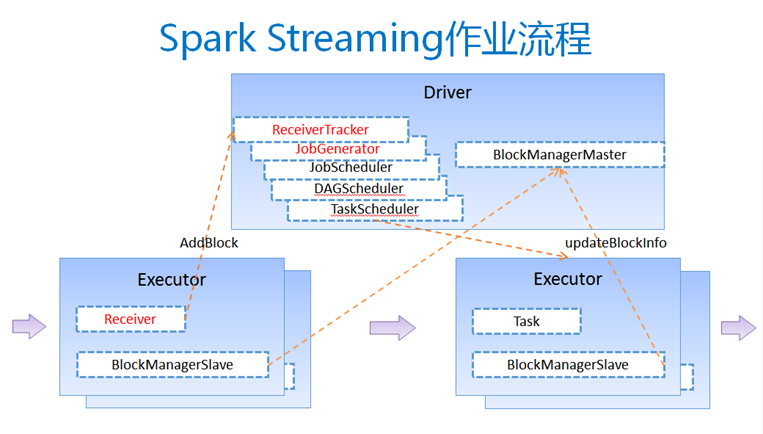
\includegraphics[scale=0.6]{spark执行流程.png}
    \caption{spark streaming执行流程}
    \label{fig:spark streaming}
  \end{figure}
 
  \begin{enumerate}[1.]
      \item  客户端提交作业后启动Driver,Driver是park作业的Master。
      \item 每个作业包含多个Executor,每个Executor以线程的方式运行task,Spark Streaming至少包含一个receiver task。
      \item Receiver接收数据后生成Block,并把BlockId汇报给Driver,然后备份到另外一个Executor上。
      \item ReceiverTracker维护Reciver汇报的BlockId。
      \item Driver定时启动JobGenerator,根据Dstream的关系生成逻辑RDD,然后创建Jobset,交给JobScheduler。
      \item JobScheduler负责调度Jobset,交给DAGScheduler,DAGScheduler根据逻辑RDD,生成相应的Stages,每个stage包含一到多个task。
      \item TaskScheduler负责把task调度到Executor上,并维护task的运行状态。
      \item 当tasks,stages,jobset完成后,单个batch才算完成。
  \end{enumerate}

\section{流式数据特征抽取}
Spark Streaming 支持 Scala、Java 和 Python,本文中使用Python提交任务。使用第三章中的特征提取方法,
输入为由kafka传入的流量数据,提取的结果都是传输层的一些统计信息,以一个TCP流或一个UDP流为一个单位。TCP流以FIN标志为结束,UDP以设置的flowtimeout时间为限制,超过时间就判为结束。在一个TCP流中有很多个数据包,先三次握手而后传输信息再四次挥手。统计一个流中的统计信息作为提取的特征。且统计的特征都分前后向,规定由源地址到目的地址为正向,目的地址到源地址为反向,为每个流构建一个标志叫Flow ID:192.168.31.100-183.232.231.174-46927-443-6,由源地址、目的地址、协议号组成。
流量特征提取的整体流程图如下:
TODO:修改图片!
\begin{figure}
    \centering
    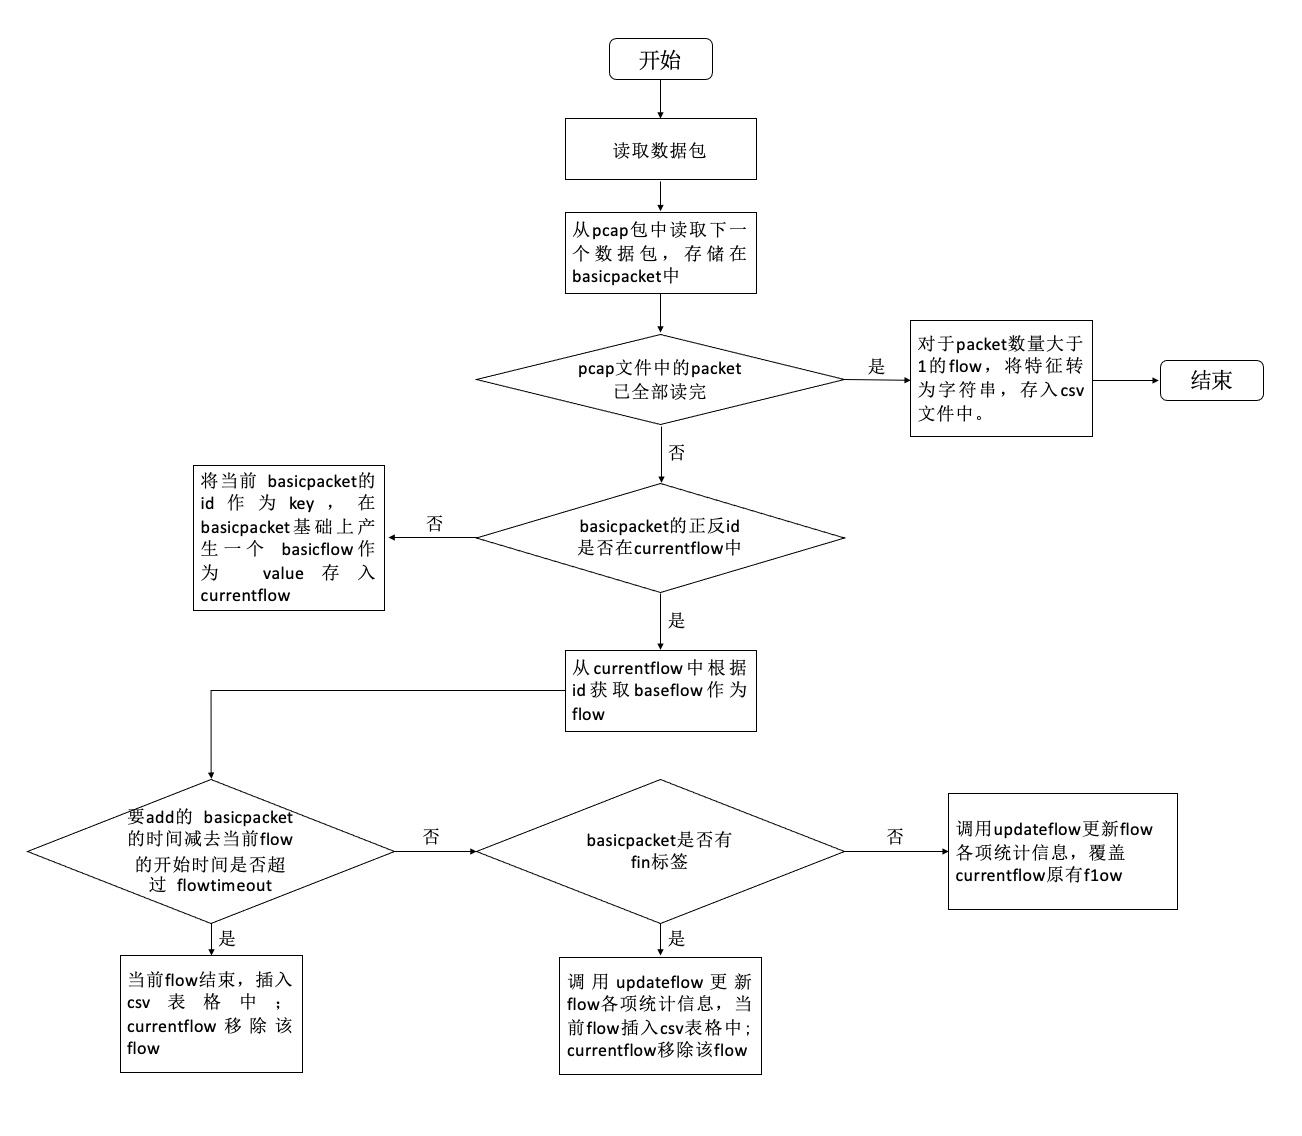
\includegraphics[scale=0.2]{特征提取.jpg}
    \caption{特征提取}
    \label{fig:特征提取}
  \end{figure}

从pcap文件中逐个读取packet,将每个数据包添加到对应的流中在currentFlows存储当前还未结束得所有TCP、UDP流。在添加的过程中不断地更新每个流的统计特征,最终将统计特征写入csv文件。判断新加入的数据包是否属于当前所有未结束的流,如果属于当前流则判断正向还是反向,之后判断时间是否超时、不超时则判断是否含有FIN标志,如果两者都不满足,则声明一个BasicFlow对象,根据id从currentFlows中拿到与当前数据包对应的流,调用addPacket将该数据包加入到对应流中。如果前面判断不在当前所有未结束的流中,则直接创建一个新得流,里面只含当前数据包,存入到currentFlows中。如果属于当前某个未结束的流,且超时或存在FIN标志,则说明当前flow结束,超时则从currentFlows中移除对应流,新建flow存入currentFlows中,含FIN标志则直接从currentFlows中移除对应流。结束的flow直接调用onFlowGenerated函数将流打印存储起来。

使用该方法得到的csv文件如下所示:
\begin{figure}
    \centering
    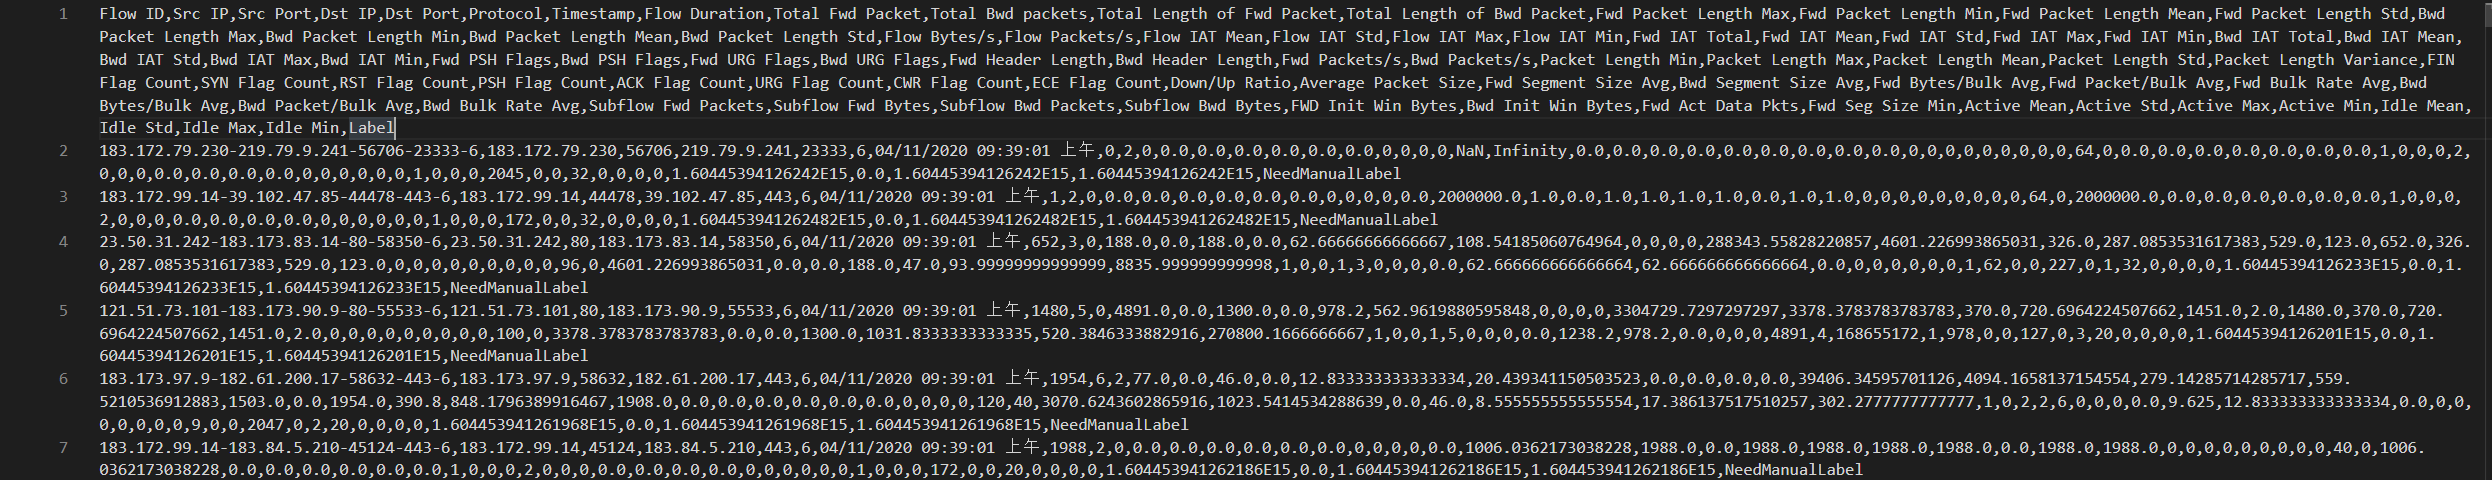
\includegraphics[scale=0.2]{特征文件.png}
    \caption{特征文件}
    \label{fig:特征文件}
  \end{figure}


\section{模型训练模块的设计与实现}
补充一些图
\section{预测输出模块}
\section{系统结果展示与分析}
本章在第二章技术分析和介绍的基础上,先后阐述异常流量检测系统的需求分析、
本文系统总体架构的设计、算法模型的设计方案,最后根据系统的总系架构和算法模型
提出本文系统五大模块的设计方案。
3.1需求分析
3.1.1功能需求分析
根据项目背景,本文设计的系统功能需求为:
(1)能够通过JnetPcap技术采集主机流量特征,采集pcap类型文件中的保存的流量特
征。
(2)能够将采集端的采集特征在后台收集端集中,过滤,写入kafka。
(3)能够对流量预测,本文将流量分成4等级,等级越高,是异常流量的可能性越大。
(4)能够对预测的结果进行良好的展示。
(5)预测模型具有一定效果。
3.1.2系统需求分析
(1)可扩展:随着后期需求的变化与增长,所以在开发过程需要考虑如何应付这些后
期变化。针对本系统,需要考虑采集模块支持Windows、Linux系统,需要考虑预测模块
中模型的更新和替换问题。
(2)健壮性:在流式处理的过程中,有可能其中一个模块偶尔发生错误,不能让这种
错误影响到整体系统运行,但是需要对这种错误进行记录。
(3)配置分离:系统的某些属性需要以配置文件的形式分离出来,方便以后对系统的
管理控制。
3.2系统总体设计
3.2.1异常流量预测系统总体架构设计
本系统属于流式系统,采集模块获取数据包流量的特征,并且实时对流量进行预测,
最后以报表的形式展示出来。结合需求和相关技术的分析,本文系统总体设计如图所
示,下面分别对各个模块的功能进行介绍。

3.2.2异常流量预测系统运行流程简介
在系统环境已经部署好的情况下,结合异常流量的总体架构设计,该系统运行的整
体流程如图3-2所示,图中编号代表这个模块运行的步骤。
% (1)训练离线模型。离线模型训练需要脱离整个数据流运行,本系统主要具有两个模
% 型,分另丨J是KMeans
% _
% RandomForest
% _
% Model和Streaming
% _
% KJVleans
% _
% Model,其中
% KMeans
% _
% RandomForest
% _
% Model基于K-Means算法和RandomForest算法实现,是监督模
% 型,需要标注数据,预测效果好;Streaming
% +
% KMeans
% +
% Modd是无监督的机器学习模型,
% 18
% 不需要标注数据,但是需要提供初始化参数,该模型预测效果不如
% KMeans
% —
% RandomForest
% —
% Model〇
(2)开启后台收集模块,收集端应该先于采集端运行,不然会导致采集端发送的数据
丢失。
(3)开启采集模块,采集并发送数据。
(4)向Spark集群提交预测模块任务,从kafka中源源不断的读取数据,并且将预测后
的结果写入一个新的kafka topic。
(4)开启报表模块展示预测结果。


